\chapter{Introduction}
\label{chap:1}
\ChapterPageStuff{1}

\section{Background}\label{section:ch1_background}
In the modern era, most businesses utilise digital products and services to maximise their profits \cite{Gralha2018}. This increases the need to create new, innovative software systems to cater to the specific needs of users. Software projects may vary in size, type, and degree of difficulty of implementation. Therefore, software quality is crucial \cite{Khan2013}. There are defined attributes and characteristics that software systems need to adhere to, which are referred to as software quality \cite{Khan2013}.\par Using a System Development Life Cycle (SDLC) methodology, such as the agile software development methodology is crucial in making the software development process efficient and predictable. This enforces various degrees of discipline to the software development process to ensure that the software quality is acceptable for the user's requirements \cite{Khan2013, Al-Saiyd2015}. Table \ref{tbl:ch1_SDLC} lists the Life-Cycle Phases (LCP) of the SDLCs.

\begin{xltabular}{\textwidth}{|l|X|}
	\caption[System Development Life Cycle phases]
	{\textit{System Development Life Cycle phases \cite{Khan2013, DOJ2003}}}
	\label{tbl:ch1_SDLC} \\
    
	\hline
	\textbf{Life-Cycle phase} & \textbf{Description} \\
	\hline
	\endfirsthead

	\multicolumn{2}{c}%
	{\tablename\ \thetable{} -- continued from previous page} \\
	\hline
	\textbf{Life-Cycle phase} & \textbf{Description} \\
	\endhead

	\multicolumn{2}{|r|}{{Continued on next page}} \\ \hline
	\endfoot

	\hline
	\endlastfoot

	\textbf{Initiation} & The sponsor identifies a need or an opportunity, creating a concept proposal for the new opportunity. This new opportunity will require a software solution to make the project successful for all stakeholders.\\ \hline
	\textbf{System Concept Development Phase} & In this phase, the feasibility and appropriateness of the concept proposal are reviewed and need approval. The Systems Boundary Document identifies the scope and requires additional approval before implementing the planning phases. \\ \hline
	\textbf{Planning} & The project management plan and other documents are created in the planning phase. These documents define the available budget, project resources, activities, schedules, tools, and reviews. \\ \hline
	\textbf{Requirements Analysis} & In this phase, the user requirements are defined and analysed. The functional requirements are created with the Functional Requirement Document. Non-functional requirements are also defined to ensure the software system operations will not deviate from working within the non-functional specifications. These non-functional requirements can be negative and costly to the software system's operations and potentially reduce its usability or life cycle. \\ \hline
	\textbf{Design} & In this stage, the detailed requirements are completed in the System Design Document, which describes the detailed logic specifications of the software system. \\ \hline
	\textbf{Development} & In this phase, the design specifications are converted into an executable software system. This also includes acquiring other third-party or internal software to install on certain software environments, creating and testing databases, performing test readiness reviews, and other software development activities. \\ \hline
	\textbf{Integration and Test} & In this phase, the software systems are integrated and systematically tested to examine if they meet all functional requirements and other accreditation activities for test approval and user approval using user tests. \\ \hline
	\textbf{Implementation} & This phase is initiated after the software systems pass the testing phase and are accepted by the users. This phase contains the implementation of the software system in a production environment and the deployment of the production version of the software. This phase continues until the software systems are operational in a final production environment.\\ \hline
	\textbf{Operations and Maintenance} & In this phase, the software system's performance is continuously monitored per the defined user requirements. Any additional modifications after the initial software development are done here, and other tasks are needed to maintain the software system. The Post-Implementation and In-Process Reviews for the software system form part of the documentation for this LCP. \\ \hline
	\textbf{Disposition} & This phase is for any disposition activities to terminate the software system properly. Any important data needed to reactivate the software system in the future is also preserved. Any other termination policies and activities should be defined and documented. This ensures that the termination of the software system is done correctly and completed and that the correct data is permanently removed or preserved. \\
\end{xltabular}

There are various adaptations of the LCP listed in \Cref{tbl:ch1_SDLC} for different SDLC methodologies used in the software development industry \cite{Al-Saiyd2015}. The planning phases of the SDLC should be well-documented, and the software architecture should be well-structured and defined to make it easier to implement the development and maintenance-related LCPs \cite{Ackermann2009}.\par Each LCP ensures that the software development is correctly implemented if it is part of the adopted SDLC methodology. The SDLC methodology is implemented for the entire software system life cycle. There will be alterations to the SDLC methodology to keep up with any new design and development requirements.\par In the actual implementation of the SDLC methodology, some design patterns may stray away from the initial software designs \cite{Reimanis2016}. This can be due to unforeseen issues during the development phase due to time or other resource constraints. The software system's initial design might also not be flexible enough for any newer modifications that can also occur in the operational and maintenance phase.\par In both situations, software development could deliver workarounds or shortcuts that resolve the identified problems. These short-term benefits will not always translate to good long-term software quality due to prioritising functionality above good software design patterns. This decreased quality of the software code is caused by technical debt if the software system was not implemented with suitable SDLC practices \cite{DeLeon-Sigg2020, Reimanis2016}.\par Technical debt can be defined as the technical compromises that software engineers and developers will introduce to a software system for short-term goals that may increase the complexity and sustainability of the system in the long term \cite{Snipes2018, Gralha2018}. With the need to always deliver software systems for more innovative, complex, and larger software systems, the risk of introducing technical debt also increases \cite{Reimanis2016, Khan2013}.\par The operations and maintenance phase of the software system is where technical debt is usually resolved or reduced to some extent. More technical debt will increase the maintenance efforts that need to be implemented to offset the negative impact that the short-term goals can potentially create. \Cref{fig:ch1_tdRepayment} represents the technical debt repayment for the software system during its entire life cycle.

\clearpage

\begin{figure}[!htb]
	\centering % cent the figure
	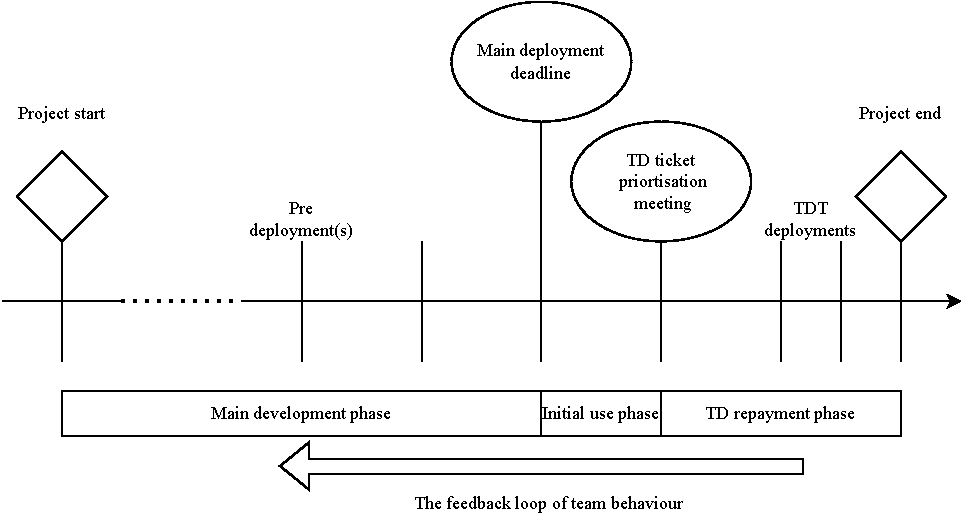
\includegraphics[width=0.9\textwidth]{img/Chapter1/TD_repayment/TD_repayment.pdf}
	\caption[Project plan with included technical debt repayment phase]
	{\textit{Project plan with included technical debt repayment phase \cite{Wiese2021}}}\label{fig:ch1_tdRepayment}
\end{figure} 

Technical debt will always be present to some degree in software systems throughout their entire life cycle \cite{Wiese2021}. In \Cref{fig:ch1_tdRepayment}, technical debt repayment refers to the software development activities that aim to resolve technical debt issues identified after the initial deployment of the software system.\par Tickets are assigned to the identified issues caused by technical debt when the functional requirements are reviewed in the initial use phase. The technical debt tickets are then prioritised based on their importance and utilisation. This ensures that the Operations and Maintenance phase development efforts are efficiently implemented for user satisfaction and the software system's sustainability.\par According to the United States Department of Commerce, software maintenance efforts of the Operations and Maintenance LCP of the SDLC in \Cref{tbl:ch1_SDLC} will contribute to about $60\%-80\%$ of the total development cost for the software system's entire life cycle \cite{Ogheneovo2014, Ackermann2009, Tang2010}. Therefore, following adequate software maintenance practices is necessary to avoid \cite{DeLeon-Sigg2020}:

\begin{itemize}
	\item additional software and hardware resources needed that can be costly,
	\item software quality issues,
	\item making any new modifications impossible without negatively impacting existing software features or systems,
	\item shortening the usability of the software system, which can lead to earlier termination of the software system.
\end{itemize}

Software maintenance of the Operations and Maintenance LCP phase is an essential task in software development. It can directly reduce the cost and effort to create new software systems or modify them in the future and reduce technical debt \cite{Thamburaj2017, DeLeon-Sigg2020}.

\clearpage

\section{State of the art}

\subsection{Software maintenance}\label{sec:ch1_softwareMaintenanceIntro}{}
Maintenance of software systems is a continuous process and a reduced form of software development aimed at modifying software systems while preserving their integrity for current and future operations \cite{Sneed2004, Ackermann2009, Port2017}. Software maintenance aims to improve the software in terms of:

\begin{itemize}
	\item \textbf{correctness:}~software systems always have some defects or faults that need to be corrected to improve their traceability, consistency, and completeness.
	\item \textbf{enhancements:}\RaggedRight~existing software components need to be improved to adapt to changes in user requirements and to improve system performance and sustainability.
\end{itemize}

A defined maintenance process needs to be followed to improve software correctness and enhancements. According to the \textit{IEEE Standard 1219}\footnote{\textbf{IEEE Standards} documents are developed within the Technical Committees of the IEEE Societies, and the Standards Coordinating Committees of the IEEE Standards Board \cite{Mamone1994}.}, software maintenance includes the following phases \cite{Mamone1994, Hasan2012, Stojanov2017}:

\begin{itemize}
	\item Identifying the problem or modification and classifying it
	\item Analysing the identification of the maintenance issue
	\item Designing the solution to implement maintenance
	\item Implementing the solution
	\item System testing of the modified software system
	\item Acceptance testing on the fully integrated system
	\item Meeting the delivery requirements of the modified software system
\end{itemize}

These software maintenance phases cannot be omitted when the software system is still active. Software maintenance needs to be implemented to ensure that the software system can keep up with defined user requirements and new user requirements in the future. This will increase the maintenance that needs to be done on both new and old systems \cite{Niu2018, Galster2019, Hasan2012}. \Cref{fig:ch1_costsOfFixingBugs} shows the representation of the total resource cost of implementing software maintenance.

\begin{figure}[!htb]
	\centering % cent the figure
	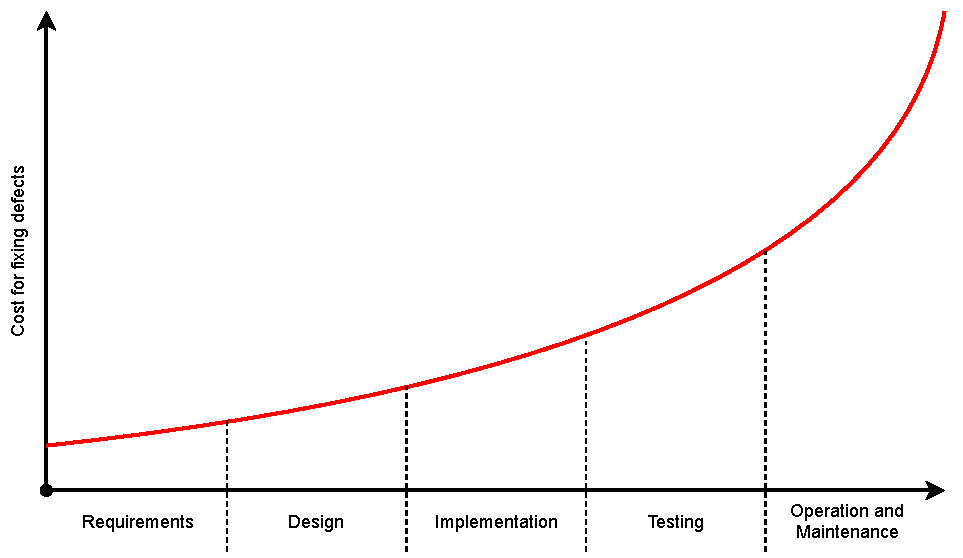
\includegraphics[width=0.55\textwidth]{Chapter1/Cost_of_fixing_bugs/Cost_of_fixing_bugs.pdf}
	\caption[Resource cost of software maintenance]
	{\textit{Resource cost of software maintenance \cite{Ogheneovo2014}}}\label{fig:ch1_costsOfFixingBugs}
\end{figure}

In \Cref{fig:ch1_costsOfFixingBugs}, the total resource cost will significantly increase as the need for software maintenance increases. As previously stated, software maintenance can use as much as $60\%-80\%$ of the total resources, and it can be expected that most of the resource costs will be for the Operations and Maintenance LCP. These software resources that cost both money and time can include:

\begin{itemize}
	\item software developers and other support staff involved in the software maintenance process,
	\item software development tools and services such as testing software environments, analysis tools, online surveys, and software fault reporting systems, etc.
\end{itemize}

\subsubsection{Software maintenance types}

Maintenance problems or modifications are regularly identified and are usually addressed based on an initial priority ranking. This priority ranking is determined by using classification models to determine which type of maintenance needs to be done, as described in \Cref{tbl:ch1_maintenanceTypes} for the Operations and Maintenance LCP of \Cref{tbl:ch1_SDLC} \cite{Tang2010, Ping2010}.

\begin{table}[!htb]
	\centering
	\caption[Software maintenance types]
	{\textit{Software maintenance types \cite{Ping2010,Hasan2012}}}
	\label{tbl:ch1_maintenanceTypes}
	\begin{tabularx}{\textwidth}{|c|X|c|}
		\hline
		\textbf{Maintenance type} & \textbf{Description} & \textbf{$\%$ of maintenance activities} \\ \hline
		Adaptive & \raggedright Adaptive maintenance in software systems is any modification or enhancements to keep it usable with a changing or changed software environment. & $\approx 37.5\%$ \\ \hline
		Perfective & \raggedright Perfective maintenance based are modifications made based on the change of the end-user new requirements. It can also improve the performance or maintainability of the software system in its life cycle. & $\approx 37.5\%$ \\ \hline
		Corrective & \raggedright Corrective maintenance are improvements made to fix certain defects or errors in a software system. & $\approx 20\%$ \\ \hline
		Preventive & \raggedright  Preventive maintenance are improvements made to software systems that prevent problems in the future. & $\approx 5\%$ \\ \hline
	\end{tabularx}
\end{table}

According to \Cref{tbl:ch1_maintenanceTypes}, adaptive and perfective maintenance types account for approximately $75\%$ of the total software development maintenance for the Operations and Maintenance LCP. These maintenance types are designed to address technical debt issues that may arise after the initial software deployment. They are typically identified through technical debt tickets, as shown in \Cref{fig:ch1_tdRepayment}. Adaptive and perfective maintenance is critical in ensuring that the software system continues to evolve and improve, meeting the system requirements to ensure that it is usable and feasible \cite{Kumar2013}.\par It is inevitable that there will always be software faults or defects that require fixing and deployment. These maintenance software changes are usually minor and aim to increase the correctness of the software system. Preventative measures may also be taken to avoid technical debt issues in the future through preventive maintenance efforts.\par However, prioritising available resources for certain parts of the software system to carry out maintenance and prevent or fix any software defects can be a challenging task \cite{Mamone1994, Hasan2012}. The defect density of a software system is determined by the number of possible defects divided by the size of the software system, as shown in \Cref{eq:ch1_defectDensity}:

\begin{equation}
	\label{eq:ch1_defectDensity}
	Defect~Density = \frac{CNDD}{KLoC},
\end{equation}

where:

\begin{itemize}
	\item $CNDD$ is the cumulative number of defects in the post-release version of the software system
	\item $KLoC$ (thousands of lines of code) is the size of the observed executable code in a software system 
\end{itemize}

A lower defect density indicates good software quality \cite{Shah2012, Alenezi2016}. However, it does not necessarily imply that the software meets all user requirements but that fewer possible faults exist.\par In open-source software systems (OSS), the defect density tends to increase due to the size of the system and the number of developers working on it \cite{Rahmani2010}. Adding more developers to improve a software system may not always lead to improvements in all maintenance types listed in \Cref{tbl:ch1_maintenanceTypes}.\par This increase in size and complexity of the software system may also lead to a higher defect density, thereby increasing the need for corrective maintenance efforts. Therefore it can further exacerbate developers' challenges as they attempt to resolve maintenance issues. \cite{SourceForged2009}.

\subsubsection{Problems with implementing software maintenance}\label{sec:ch1_maintenanceProblems}
Under most circumstances, maintenance is implemented if a software system does not meet the required functions specified by the user or performance requirements \cite{Ogheneovo2014, Sneed2004}. Maintenance can be difficult to implement due to the following:

\begin{itemize}
	\item \textbf{Problem domain being complex:} The software may not be well defined or structured during the planning LCP phases of \Cref{tbl:ch1_SDLC}. This is due to how large the software systems grow over their entire life cycle or duplicate software components that are made.\par A poor understanding of the system architecture or insufficient documentation about the software system exists when analysing the maintenance issues \cite{Galster2019}. Software engineers and developers tend not to create or update documentation as it is time-consuming when software needs to be delivered on schedule.
	\item \textbf{Difficulties of managing development process:} Most companies will strive to increase their digital products and services over the life cycle of the software project to maximise possible profits with the resources invested \cite{Niu2018}. Increasing production of the development process will only strain the maintenance efforts of the software systems \cite{Sneed2004}.\par Software engineers and developers already have a busy schedule to deliver software features on time \cite{Galster2019, Lenarduzzi2017}. They will quickly feel overwhelmed and suffer from development burnout if the development process is not correctly managed to include additional software development by implementing maintenance.
	\item \textbf{Flexibility of the software:} Trying to predict what the future architecture may look like and modify it while preserving the software's integrity may be difficult in software maintenance \cite{Garlan1999}. Software is flexible if it is adaptable to the problem domain when adding modifications to it \cite{Ogheneovo2014}.\par Most development teams will follow a software development methodology to create a future architecture that is modular and structured to preserve the development integrity of new software \cite{Vijayasarathy2016}. This will also have an impact on the type of maintenance activity (as in \Cref{tbl:ch1_maintenanceTypes}) the development team will need to implement \cite{Thamburaj2017, Snipes2018}.
	\item \textbf{Change in user's requirements:} In software development, the users will often request new additional requirements to the software systems delivered to them \cite{Ogheneovo2014}. Modifying software systems may include new and additional features that change the initial system architecture. Maintenance of these systems is crucial to ensure that existing components of the system will work as intended with the new components that are added.
	\item \textbf{Environmental changes:} Rapid changes in software development are always present, with the need for more innovative solutions added to solve new complex problems. These changes are not always compatible with existing software systems even if the initial software architecture is well-defined \cite{Ogheneovo2014}. \par There will always be a need to make improvements to the software system in the form of third-party software updates and services used. The software system needs to be modified to accommodate these new changes as it is beneficial for its sustainability and operation.
	\item \textbf{Bad design:} Maintenance can be difficult if the system is badly designed when the SDLC was implemented. The maintainability of the system is impossible or too difficult without making major changes. The complexity of the software system may be too high for some developers which will cause the mentioned problem domain issue with complexity in software systems \cite{Lenarduzzi2017}.
\end{itemize}

\clearpage

\subsubsection{Software maintenance prioritisation}\label{sec:ch1_maintenanceModel}
Due to time constraints and available resources, it is difficult to plan any maintenance operations for most software engineers and developers \cite{DeLeon-Sigg2020}. The increased resource cost of software maintenance is due to a lack of planning or preventive measures to keep the software system from degrading \cite{Alenezi2016}.\ Continuous par analysis of the identified maintenance problems or modifications enables the software engineers and developers to create a preliminary plan to address these issues efficiently \cite{Port2017}. Implementing a suitable maintenance framework to resolve the identified issues reduces technical debt.\par Various maintenance models can be used to solve these issues when implementing any of the maintenance types. A software maintenance model is an abstract representation of software systems' evolution to keep track of all the maintenance activities when implementing software maintenance \cite{Ren2011}. The \textit{IEEE Standard 1219} for software maintenance is the standard that should be followed when planning software maintenance as in \Cref{fig:ch1_ieeeModel}. 

\begin{figure}[!htb]
	\centering % cent the figure
	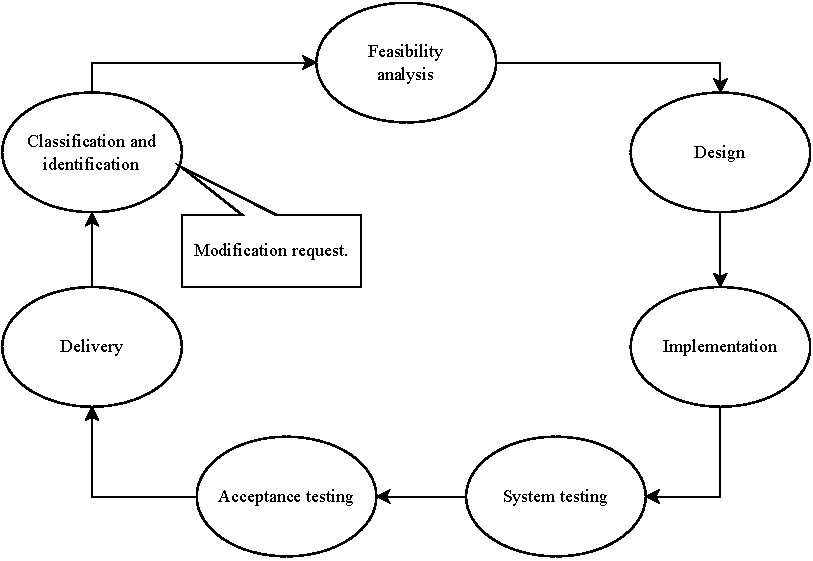
\includegraphics[width=0.65\textwidth]{Chapter1/IEEE_Model/IEEE_Model.pdf}
	\caption[IEEE Standard 1219 model for software maintenance]
	{\textit{IEEE Standard 1219 model for software maintenance \cite{Ren2011}}} \label{fig:ch1_ieeeModel}
\end{figure}

The software maintenance model in \Cref{fig:ch1_ieeeModel} emphasises that software defects or faults must be identified and classified for maintenance. A feasibility analysis of any required changes should be made if the maintenance effort is worth implementing. A certain amount of resources will be allocated to implement maintenance, impacting the design and implementation phase.\par For the feasibility analysis, making use of a system characterisation report may help identify possible maintenance focus points in a software system \cite{Araujo2021}. This will increase the effectiveness of designing solutions to implement maintenance as a system assessment focus can be made. The metrics can be defined as:

\begin{itemize}
	\item positively or negatively impacts the performance of the system,
	\item fulfil the defined user's requirements,
	\item increase user engagement with the defect and fault fixes or expand existing software components with additional features,
	\item is worth a large portion of the user base to implement.
\end{itemize}

User engagement with the software system is what will determine if the software system is sustainable in generating revenue for the organisation. It may be the most crucial focus metric for the feasibility analysis to determine if a maintenance effort is worth implementing \cite{Araujo2021}. Compared to the one in \Cref{fig:ch1_maintenanceFlow}, a maintenance flow model can resolve this issue.  

\begin{figure}[!htb]
	\centering % cent the figure
	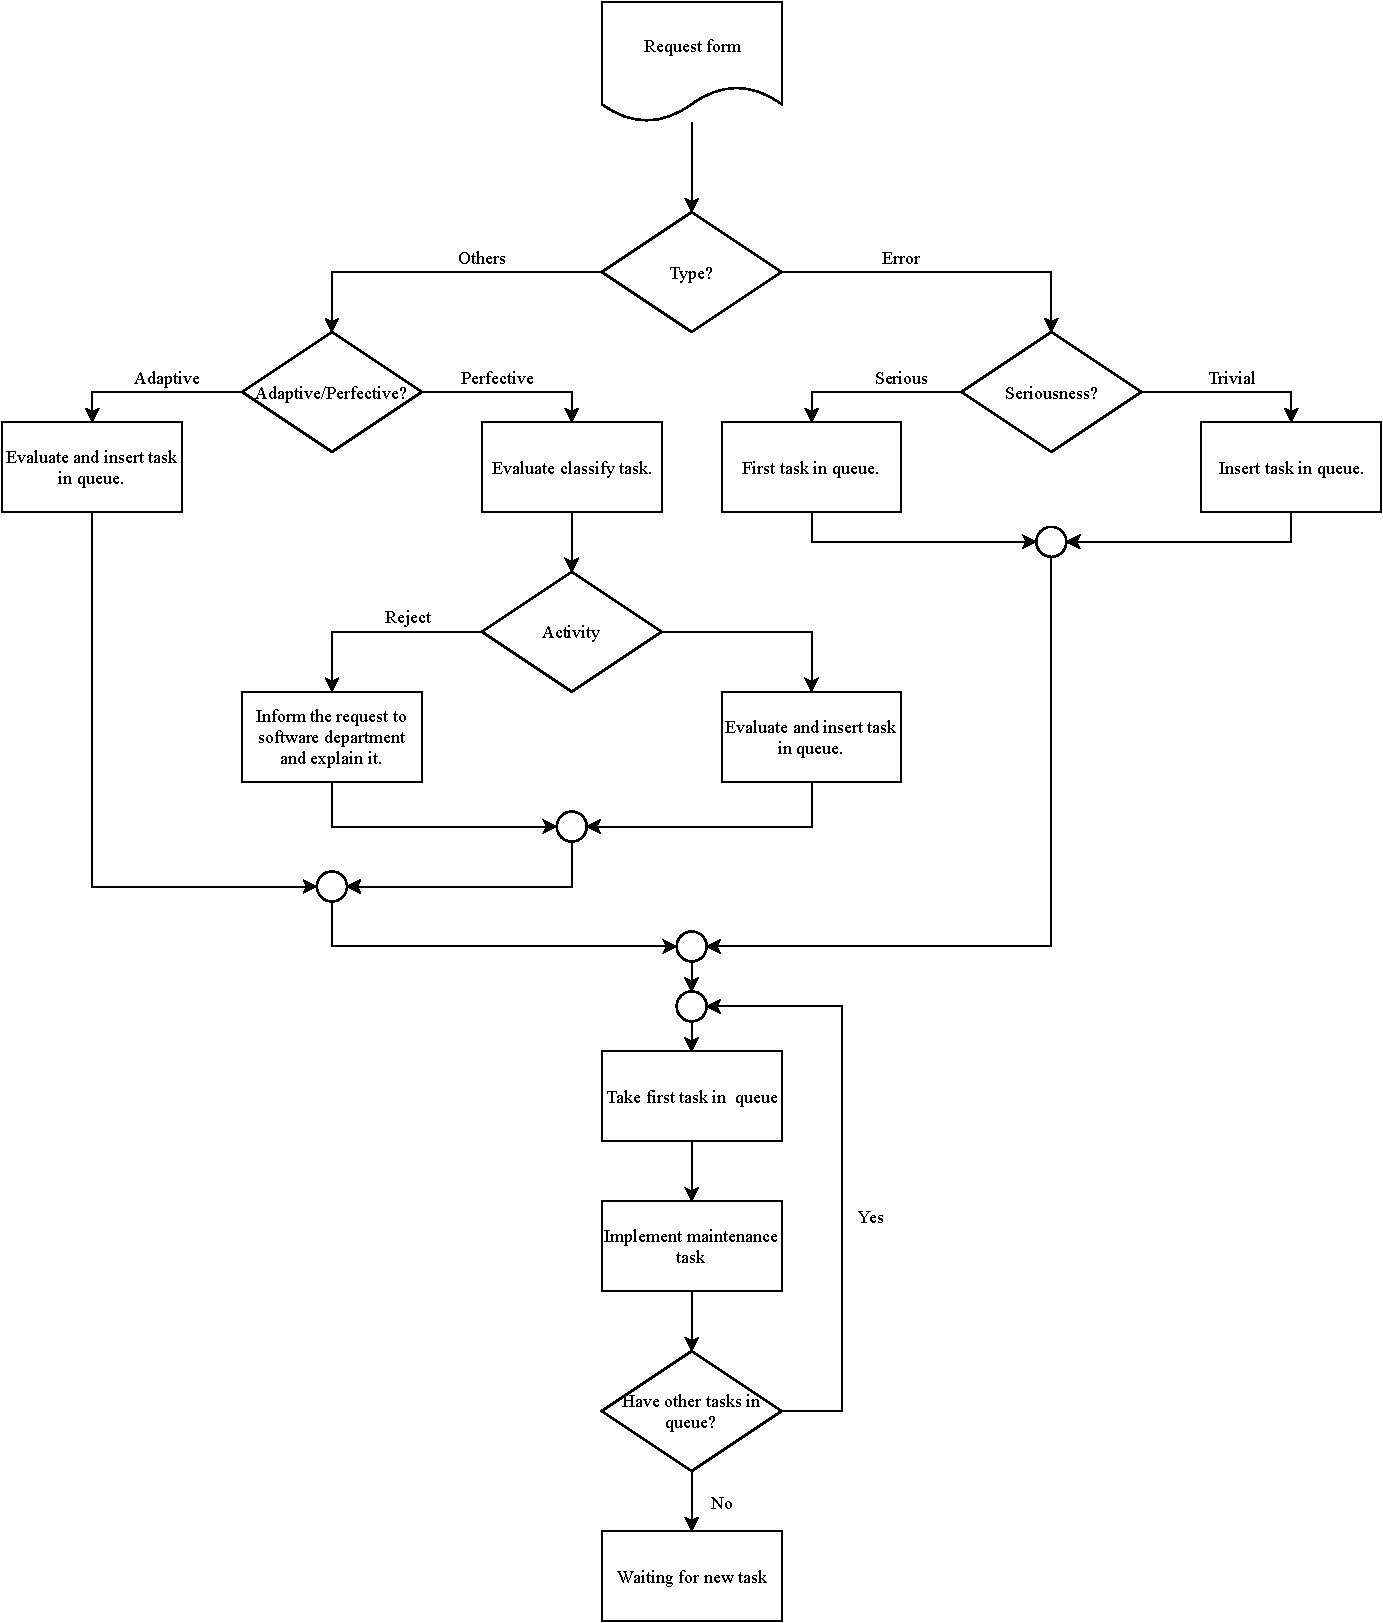
\includegraphics[width=0.95\textwidth]{Chapter1/Maintenance_flow/Maintenance_Flow.pdf}
	\caption[Maintenance flow model]
	{\textit{Maintenance flow model \cite{Tang2010}}} \label{fig:ch1_maintenanceFlow}
\end{figure}

\Cref{fig:ch1_maintenanceFlow} is an example of what a practical maintenance flow model is an organisation would likely use to implement software maintenance. Initially, a developer will complete a request form or issue indicating a new problem or feature request that needs to be implemented \cite{Tang2010}.\par After all the maintenance tasks are defined, the development team will prioritise the higher-rated issues that need to be solved. This process will repeat itself until all the task for that specific software system is completed.\par To fully follow the \textit{IEEE Standard 1219} of implementing maintenance on a software system, the defects or areas of improvement should be identified. Utilisation analysis of event logs can be used to detect any hidden defects or performance issues in a software system to implement software maintenance \cite{Cinque2013, Rong2018a, Levin2019}.\par System and acceptance testing are essential to ensure that the system is still fully functional and fulfils the user's requirements. After the system is thoroughly tested and approved, it will be available to the user, and the maintenance process will start again when there are new improvements to be made to the software system.\par In \Cref{sec:ch1_softwareMaintenanceIntro}, it was identified that software maintenance is essential to be able to fulfil the user's requirements. For any maintenance model, as described in \Cref{sec:ch1_maintenanceModel}, to be effective, the software maintenance model will need to be able to prioritise the maintenance issues efficiently. \par Most organisations' maintenance models will be based on \Cref{fig:ch1_ieeeModel} to manage their Operation and Maintenance LCP maintenance efforts. Up to $50\%$ of a software engineer or developer's total time invested in implementing maintenance is to understand what the software system is supposed to do \cite{Tang2010}. This is due to the problems with implementing maintenance as discussed in \Cref{sec:ch1_maintenanceProblems}.\par If the issue is a problem in the software system, the severity of the problem needs to assess to decide on the priority level to resolve it. This type of maintenance is mainly corrective and can also be preventive if it is a possible solution to prevent any software failures in the future \cite{Tang2010}. Other types of maintenance requests are either adaptive or perfective and usually placed in the development team's task queue. \par Prioritising maintenance for the user's requirement to extend usability and increase user satisfaction is preferable to maximise profits. In most cases, when no suitable software maintenance model is used, the software maintenance is reactive \cite{Araujo2021}. However, this is not a sustainable maintenance policy for larger, more complex software systems. \par To prioritise maintenance more efficiently, a system characterisation of the software system needs to be made. In \Cref{sec:ch1_maintenanceModel}, user engagement with the software system has been identified to be an important metric when implementing maintenance.\par Knowing what the user uses or how they interact with the software system provides valuable data to the development team. But to access that data, some form of tracking is needed to obtain the data automatically.


\clearpage

\subsection{Event logging}\label{sec:ch1_eventLogging}
As described in \Cref{sec:ch1_maintenanceModel} a tracking method is needed to capture data about user engagement with the software system for maintenance purposes. It is a common practice in the software industry to record any detailed system run-time information into event logs. These event logs can be analysed later by developers or software engineers to solve software-related problems \cite{Zhu2019}. \par Event logging is a proven implementation to get information about the behaviour of software systems \cite{Baccanico2014}. Event logs are software system-generated textual files that collect data on reported events of interest that occur during various operations of the software system. \cite{Cinque2013, Baccanico2014}.\par The technique to collect numeric or textual data that describes the behaviour of a computer system is called event logging \cite{Pecchia2015, Baccanico2014}. Event logs collect textual data containing the records of events that happened in a software system and are used for system management tasks as in \Cref{tbl:ch1_eventLogsUsage} \cite{Rong2018a, Rong2018, Baccanico2014}. Event logging has three major purposes \cite{Pecchia2015, Baccanico2014}:

\begin{itemize}
	\item \textbf{state dump} is reporting of values of certain variables or data structures inside the software system.
	\item \textbf{execution tracing} is the reporting of certain states of the software system or what is currently happening in the software system,
	\item \textbf{event reporting} focuses on any desired events in the software system that has textual information of that event.
\end{itemize}

Event logs are mainly used for event reporting to support debug and system integration activities to reduce the amount of code that needs to be inspected \cite{Baccanico2014}. \Cref{tbl:ch1_eventLogsUsage} is the most common use of event logging in the industry is described.

\begin{xltabular}{\textwidth}{|l|X|}
	\caption[Event logs usage]
	{\textit{Event logs usage}}
	\label{tbl:ch1_eventLogsUsage} \\
    
	\hline
	\textbf{Usage} & \textbf{Description} \\
	\hline
	\endfirsthead

	\multicolumn{2}{c}%
	{\tablename\ \thetable{} -- continued from previous page} \\
	\hline
	\textbf{Usage} & \textbf{Description} \\
	\endhead

	\multicolumn{2}{|r|}{{Continued on next page}} \\ \hline
	\endfoot

	\hline
	\endlastfoot

		\hline Debugging of software systems and services & Event logging is mostly used to record events or behaviours of software systems or services during its run-time \cite{Rong2018a}.\\
		\hline Anomaly detection & Event logs can be used to detect any abnormal system behaviour using an anomalous detection algorithm using logging data \cite{Gurumdimma2016}. This can also be used to find any potential vulnerabilities or defect prediction in the software environment \cite{Dwyer2013}. \\
		\hline Performance diagnosis & Software performance is important to producing quality software for the end user \cite{EvangelinGeetha2007, Baccanico2014}. This is also important to make informed decisions on how to improve the software system or service for improved performance and other resource and financial implications.\par This type of performance event logs of the software systems or services are used to monitor the software system, which is useful for resource tuning, load balancing and checking system scalability in the entire life cycle of the software system or service \cite{Song2017}. \\ 
		\hline Auditing & In a software environment there can be significant changes to the database data that might need to be logged for auditing purposes \cite{Rong2018a}. All establishments and enterprises need to ensure that compliance with the industry regulations is met with their software systems by adding audit logs. They are also legally bound to have audit logs to provide legal evidence for any legal investigation or administrative tasks to ensure that accountability is maintained. \\
		\hline Error and failure analysis & Event logs are used to analyse the failure behaviours of software systems which enable software engineers or developers to understand the failure modes of the system, find the root cause of these failures, prevent them and improve the reliability of the future releases of the system \cite{Cinque2013}.\\
		\hline Analysis of security alerts & In any software environment or information technology infrastructure, security is a major concern for any organisation \cite{Pathan2014, Dwyer2013}. It is important to know the overall security status of the software system. \\
\end{xltabular}

\paragraph{Logging practice in software development}\label{sec:ch1_loggingPractice}\leavevmode\\
Logging practice in software development is not always well documented, and there can be multiple implementations of different logging mechanisms in the same software system \cite{Pecchia2015, Kitchenham2007}. In modern software systems, the logging practice is a crucial part of the development of software and the maintenance of it in its entire life cycle \cite{Rong2018}.\par In \Cref{apx:loggingPractice} there has been a rise of new studies that focus on providing suitable logging practice guidelines to software engineers and developers. Logging in the industry makes use of many third-party logging libraries and frameworks such as Apache's log4net and Microsoft's ULS frameworks \cite{Zhu2015, Rong2018}.\par Software engineers and developers can use these tools to implement logging in a compatible software system. They will still need to know how to strategically place the logging points so that the desired logs can be obtained. Using guides provided by the tools and other online guides, the logging practice can be implemented. When using a third-party logging mechanism, the software engineers and developers will, in most cases, need to:

\begin{itemize}
	\item add the logging points in the software system at locations where it can capture the desired logs,
	\item enables the log parsing stage to write a log entry into a database.
\end{itemize}

Logging guides can give examples and suggestions on where to place the logging points but that can still be difficult on occasion for software engineers and developers to identify these desired locations. This can be difficult due to logging guides being mostly application-specific or the logging mechanism can only capture certain event types to create event logs. \par For more custom logging, the software engineers and developers will need to create new logging mechanisms. This adds new requirements for the logging mechanism to be functional. For a logging practice to be successful, two important problems need to be resolved \cite{Zhu2015, Zhu2019, Rong2018}:

\begin{itemize}
	\item \textbf{What needs to be logged?}\par In \Cref{tbl:ch1_eventLogsUsage} the use of logging is diverse and will have an impact on how the logging mechanism will be designed.
	\item \textbf{Where to log?} \par Different types of logs will only be present in the software system at certain locations during run-time. Knowing what to log narrows down which locations can be used to obtain certain events while they are present.
\end{itemize}

To answer these two questions the event log has to fulfil certain log quality requirements. This ensures that the created logs are correct and consistent when it is extracted and viewed. 

\clearpage

\subsubsection{Logging quality}\label{sec:ch1_loggingQuality}

Software engineers and developers will need to make informed logging decisions for event logging. These decisions may affect the software system's run-time operations negatively and can impact the event logging efficiency \cite{Zhu2015, Zhu2019, Kherbouche2017}. An event log quality model in \Cref{fig:ch1_EventQModel} can be used define to ensure that the event logs will have consistent integrity when capturing the event log data.

\begin{figure}[!htb]
	\centering % cent the figure
	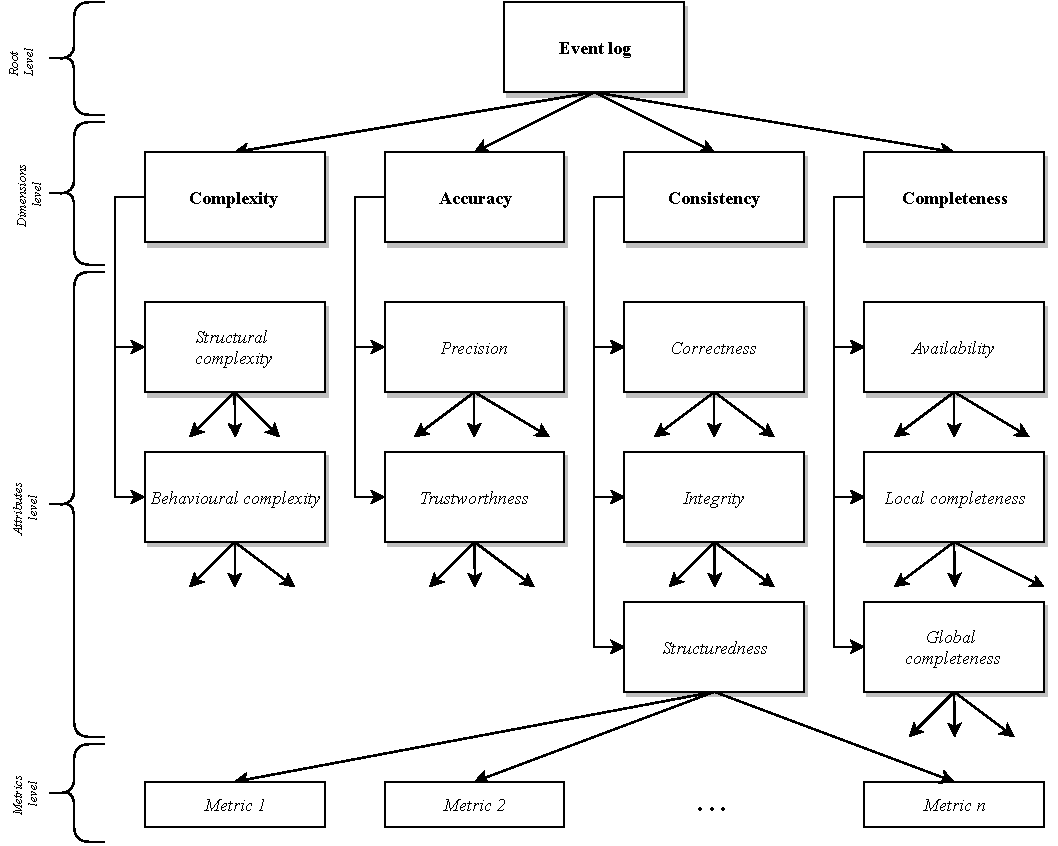
\includegraphics[width=0.99\textwidth]{Chapter1/Event_Log_Model/Event_Log_Model.pdf}
	\caption[The event log quality model]
	{\textit{The event log quality model \cite{Kherbouche2017}}} \label{fig:ch1_EventQModel}
\end{figure}

The event log quality model in \Cref{fig:ch1_EventQModel} consists of four different levels to define each property of the event log quality model:

\begin{itemize}
	\item Root level for the event log quality model. These are the main requirements for the event log quality model,
	\item Dimension level which consists of four main dimensions of the event log quality model according to \cite{Kherbouche2017} (complexity, accuracy, consistency and completeness of the event log),
	\item Attributes level where a set of quality attributes for the dimension level,
	\item Measurement level which should be defined in the design process of the logging mechanism to achieve the attributes and dimension levels.
\end{itemize}

\clearpage

\begin{itemize}
	\item \textbf{Accuracy of event logging}\par It can become difficult to log every event in a software system as these systems will get larger and more complex during their development life cycle \cite{Stojanov2017}. Precisely capturing certain events that need to be logged needs to be consistent to ensure that the data is trustworthy and reliable to use. The log attributes of the event log also need to be precisely captured for each event log and should be correct.\par Capturing more event logs doesn't guarantee that the accuracy of the event log is on an acceptable level as the log's attributes can be incorrect or cause duplicated events logs if the data is the same in a sequence of event logs. In \Cref{tbl:ch1_loggingTooMuch} are the common problems associated with too much logging.

	\begin{table}[!htb]
		\centering
		\caption[Problems with too much logging]
		{\textit{Problems with too much logging \cite{Zhu2015}}}
		\label{tbl:ch1_loggingTooMuch}
		\begin{tabularx}{\linewidth}{|l|X|}
			\hline \textbf{Problem}  & \textbf{Description} \\
			\hline \textbf{Excess code} & Adding multiple logging points may increase the amount of code added to the software system to capture the event logs. The code may take some time to write and maintain. This can increase the structural and behavioural complexity of the code in its entire life cycle. \\
			\hline \textbf{System resource impact} & With the additional code needed to capture the logs the system resource usage such as the CPU and I/O channels will increase. This may negatively impact the performance of existing system operations or increase the cost to keep the system at the same operation speed by increasing the system resources.\\
			\hline \textbf{Unusable logs} & Adding numerous logging points or logging too much at points can produce numerous trivial or useless logs that will not improve the system utilisation analysis. When implementing the system utilisation analysis stage the logs might need to get filtered more or modified to be more meaningful as much as $70\%$ of the logs may be irrelevant \cite{Fedaghi2010}. \par The logs are written by the software engineers and developers and can sometimes be irrelevant to other managers or system administrators when implementing a log analysis report of the event logs. More event logs can have missing or incomplete logging attributes due to the excessive logging points that have been added. The increase in the behavioural complexity of the log can impact the decisions that are made to improve software maintenance. \\
			\hline
		\end{tabularx}
	\end{table}

	The accuracy and trustworthiness of the event log are more important than capturing a large number of available event logs in a software system \cite{Zhu2015, Jans2012}. The extra unnecessary logs will also take up more storage space store which will increase costs and possibly the performance of the software system. 

	\item \textbf{Event log complexities}\par Software always has some complexity involved and it will always increase when the software system becomes larger. For the event log quality model the complexity of the event can be split into two different complexities which are \cite{Kherbouche2017}:

	\begin{itemize}
		\item Structural complexity is the application of different algorithms in the software which allows the event log to be evaluated when it occurs which can alter the behaviour of the event log.
		\item Behavioural complexity in event logging is the complexity of the behaviour of the event logs that refers to the number of smaller events in each captured trace and the different variations of these traces within an event log.
	\end{itemize}

	These two complexity attributes can be costly when the event logging mechanism needs to be constantly maintained in large software systems where it can impact the rest of the system's performance or integrity of the captured event logs \cite{Ogheneovo2014}. The constant modification of the event log software can be due to technical debt as the event log system's complexities lead to technical issues when attempting to log an event or are not compatible with other systems \cite{DeLeon-Sigg2020}.  

 	\item \textbf{Consistency of event logging}\par The event logs' accuracy and consistency are critical when making reliable decisions based on the identified behaviour of the software system with the historical data that exists in the event logs that are discussed in the previous event log quality dimension \cite{Stojanov2017, Kherbouche2017}. With the accuracy and trustworthiness of the event logs correctly applied, the consistency of the event logs should be on an acceptable level to be correct and verifiable when comparing it to the software system. \par An event log quality model is essential to ensure that the logs will be of high quality for the data mining process of log analysis and therefore the event log data should be consistent. To ensure the consistency of the event logs the structure of the event logging points and log parsers should be consistent to capture all the important log attributes. The event log data should also be consistently analysed with different methods used on it as part of the consistency of the event logging process.

	\item \textbf{Completeness of event logging}\par The event logs will be analysed at a later stage, the logs should be fully complete when it is being used as some of the other logging attributes might not be available at that stage. The event logs' available attributes should be accurately captured before attempting to store them in a database to ensure that there is no missing event data or missing events if the event is discarded due to it being incomplete. There are two types of completeness attributes excluding the availability attribute in the \Cref{fig:ch1_EventQModel}:

	\begin{itemize}
		\item Local completeness refers to all event data that can be captured for an instance of the event taking place that can be added as a log attribute to the event log \cite{Kherbouche2017, VanDerAalst2004}.
		\item Global completeness refers to the occurrence of all possible outcomes or behaviours of the event logs that can be captured which is required for the system utilisation analysis \cite{Kherbouche2017, VanDerAalst2004}.
	\end{itemize}

	Ensuring that both completeness levels are achieved and that the event log data is complete can impact performance if certain data is not directly available during the instance when the event has occurred. The logging mechanism needs to capture this as efficiently as possible without causing performance issues to the rest of the software system's operations \cite{Zhu2015, Zhu2019}. 
\end{itemize}

\subsubsection{Logging parsing and log points}\label{sec:ch1_loggignPoints}
Knowing what to log can significantly reduce any overhead the logging mechanism may produce in the software system \cite{Jia2018, Pecchia2015}. Preserving quality (as described in \Cref{sec:ch1_loggingQuality}) is a necessity to ensure that the logs that are obtained will fulfil their purpose when analysing it.

\paragraph{Logging attributes}\leavevmode\\
Before the logs can be parsed to a structured data set the key attributes that need to be defined that will describe the event log \cite{Bekeneva2020}. The attributes in describing in \Cref{tbl:ch1_logBasicAttributes} are the most basic attributes a log event should have. 

\begin{table}[!htb]
	\centering
	\caption[Basic log event attributes]
	{\textit{Basic log event attributes \cite{Bekeneva2020}}}
	\label{tbl:ch1_logBasicAttributes}
	\begin{tabularx}{\textwidth}{|c|X|}
		\hline \textbf{Attribute} & \textbf{Description} \\
		\hline Case number & Unique identifiers for each log event. This is usually the primary identifier for the log event. \\
		\hline Timestamp & The time and date that the log event occurred. This is part of identifying the order of events or traces along with the case number of the event log \cite{Kherbouche2017}. \\
		\hline Event type & Each log event can be grouped with other log events that have similar actions that happened. These event-type attribute needs to be classified based on a state change, failure to execute an instruction, or due to an occurrence of activity like the availability of service \cite{Fedaghi2010}. \par The event type is usually also the log level. The log level in event logging reflects the severity of the event log \cite{Rong2020}. An event of interest may have different log levels and this makes it easier to capture certain events in which software engineers and developers are interested.\\
		\hline Originator & The origin from which the event took place in the software system. This can be parts of the software that performs the event action or was the cause for the event to be initiated by another part of the software. \\
		\hline Other metadata & This is any other relevant information that can be used as the event log's attribute that further expands the information of the log event. This can be one extra field or many other individual attribute fields.\\
		\hline
	\end{tabularx}
\end{table}

These attributes make it possible to mine and analyse the logs based on their attributes and increase the precision and reliability of the event log \cite{Kherbouche2017}. The case number and timestamp attributes in \Cref{tbl:ch1_logBasicAttributes} can be defined anytime during the logging process. This is not the case for the rest of the attributes.\par Every log should have a defined action that will put it in a group of logs that can be defined as the event type. These event types can be either predefined of what is expected from the event action or will need to be observed later analysis of the logs in case there is no clear grouping of the logs \cite{Bekeneva2020, Fedaghi2010}.

\paragraph{Log points}\leavevmode\\
The sources of the log event assist on determine the location where the event took place. For event logs, it this essential to try to recreate scenarios or actions based on the relevant parts of the software system that participated in the event action.\par Other metadata can increase the log quality by providing additional information about software instructions that were executed. These attributes add more information that can be used to recreate the scenario or action that may be unique parameters or other events that participated in the event log.\par To get the attributes in \Cref{tbl:ch1_logBasicAttributes} an instruction generates the log and parses it onto a data set. These log instructions are called logging points in the software environment \cite{Pecchia2015, Zhu2015}. They can be any instruction such as a print function that displays the information for the user to more complex functions or libraries that can be created by third-party developers. In \Cref{fig:ch1_logParsing} is an example of a logging point parsing a log message in a structured log. 

\begin{figure}[!htb]
	\centering % cent the figure
	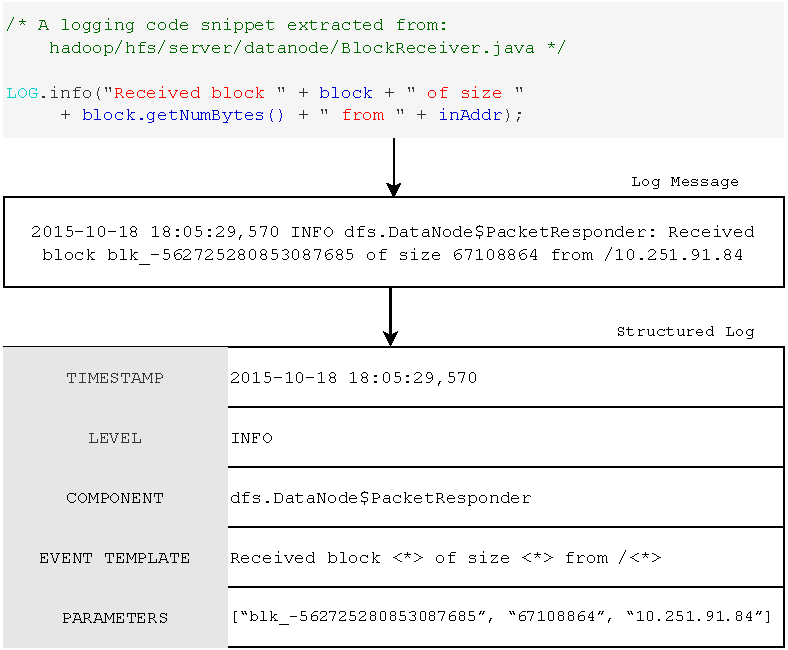
\includegraphics[width=0.95\textwidth]{Chapter1/Log_Parsing_Example/Log_Parsing_Example.pdf}
	\caption[An illustrative example of log parsing]
	{\textit{An illustrative example of log parsing \cite{Zhu2019}}} \label{fig:ch1_logParsing}
\end{figure}

The defined attributes are captured by the logging point when the event takes place or occurred. The created log message is then parsed into a structured log to be safe in a database or displayed. The logging point should be strategically placed to capture the required attributes to complete the log event \cite{Fedaghi2010}.\par Determine where to place the logging point in a giving software is directly impacted by what the attributes are and if the captured log will be of high quality as described in \Cref{sec:ch1_loggingQuality}. The availability of consistent high-quality logs will directly impact the process mining in the analysis of the logs \cite{Kherbouche2017}.\par To strategically place a logging point developers needs to consider what the activation of the logging point will be during the run-time of the software system \cite{Pecchia2015, Cinque2013}. The activation can be simple if a statement meets certain criteria or instructions that execute after when an event or action took place (e.g. run-time errors). \par The log level or event type of \Cref{tbl:ch1_logBasicAttributes} can be used to determine where the log points should be placed. The aim of the placement of the logging point should try to capture all the log attributes when the event of interest has happened.

\subsubsection{Log analysis in Web-based applications}
With the defined log parsing and log points in \Cref{sec:ch1_loggignPoints} a log analysis can be made from the stored event logs. The log analysis is the data mining process focused on the software system's generated event logs \cite{Slaninova2014,Hasiloglu2018}.\par The log analysis will make use of the defined log attributes in \Cref{tbl:ch1_logBasicAttributes} to complete it. Each software system will have some variation of the log attributes in \Cref{tbl:ch1_logBasicAttributes}. For a Web-based application, the log attributes will also contain any data about the requests between a web server and web client and its responses \cite{Slaninova2014, Dhanalakshmi2016}. This will also reflect on the log level at which weblogs are obtained for log analysis.


\subsection{Log analysis}\label{sec:ch1_systemUtilisation}
In Web-based applications, the process to get usage statistics and user behaviour data is called Web analytic \cite{Kocsis2012}. Web analytics can be used for user modelling efforts and is a form of log analysis. User modelling in software engineering is the customisation and adaptation of the software systems to the users' required needs \cite{Waqar2017, Paliouras1999}.\par The user modelling can also include the implementation of software maintenance as the maintenance is an adaptation of the software system to the user's needs which is the utilisation analysis using event logs. Web analytics focuses on different analytics in \Cref{tbl:ch1_webAnalytics} for the analysis. 

\begin{table}[!htb]
	\centering
	\caption[Web analytic for user-based data]
	{\textit{Web analytic for user-based data}}
	\label{tbl:ch1_webAnalytics}
	\begin{tabularx}{\textwidth}{|l|X|}
		\hline \textbf{Analytic}  & \textbf{Description} \\
		\hline \textbf{Identity of the user} & This is any information about the user's identity in the software system. Users can have different roles when using the software system such as a system admin or general user. These roles mostly dictated what the user can access and do on a website. \\
		\hline \textbf{Site interaction} & The different Web sites the user is accessing during their active Web session. This would also contain all the information about: 
		\begin{itemize}
			\item how often the users visit a website,
			\item how much time they spent on a specific website,
			\item navigation between different web pages of the website.
		\end{itemize}
		\\
		\hline
	\end{tabularx}
\end{table}

These same analytics can be used for none Web-based applications as the: 
\begin{itemize}
	\item identity of the user can be captured if the software system uses a software license,
	\item different parts of the system can be tracked or services that are used by the user.
\end{itemize} 

\subsubsection{Analytic tools for event logs}
There exist numerous third-party analytic tools for event logging data monitoring and management to graphically visualise the log data. Choosing the correct tool to use can be dependent on what the software engineers and developers want to analyse and the availability of the tools due to external factors like cost and usability. \par Event logging monitoring and management tools are sometimes underutilised and are not often used to their full potential when analysing the event logs \cite{Fedaghi2010}. This can be due that the log quality of event logs doesn't meet the standards of \Cref{fig:ch1_EventQModel} not met in \Cref{sec:ch1_loggingQuality} for the correct logs to be available for the system utilisation analysis. 

\clearpage

\subsection{Gap identification}
In \Cref{section:ch1_background} the importance of software maintenance is discussed in the background and that system utilisation is needed to assist with the software maintenance efforts.

\subsubsection{State of the art topics}
From the literature, there were a few important focus points identified to create a logging mechanism for user-based activities. These focus points exist for the research done in \Cref{sec:ch1_softwareMaintenanceIntro,sec:ch1_eventLogging,sec:ch1_systemUtilisation}.\par The research for this study focused on published accredited, peer-reviewed journals or articles for the last two decades (2000-2022). Some exceptions are older than 20 years as software maintenance is an essential part of modern software development for the last few decades. These studies were obtained from the IEEE Digital Library in journals by focusing on three key topics: \textbf{software maintenance}, \textbf{event logging} and \textbf{log analysis}. Each of the three main states of the art topics is divided into subtopics that explore different studies that are relevant to the main topic.

\paragraph{Software maintenance} \leavevmode\\
Software maintenance implementation in industry and best practices when implementing software maintenance subtopics are described in \Cref{tbl:ch1_soaSoftwareMaintennace}.

\begin{table}[!htb]
	\centering
	\caption[Software maintenance state of the art sub topics]
	{\textit{Software maintenance state of the art sub topics}}
	\label{tbl:ch1_soaSoftwareMaintennace}
	\begin{tabularx}{\linewidth}{|l|X|X|}
		\hline \textbf{Topic}  & \textbf{Description} & \textbf{Evaluation criteria}\\
		\hline Types and implementation & \RaggedRight Software maintenance types and implementation in industry. & \RaggedRight \begin{enumerate}
			\item Did the study focus on software maintenance?
			\item Did the study discuss different software maintenance types or implementations?
		\end{enumerate} \\
		\hline Problems & Challenges with implementing software maintenance. & \RaggedRight \begin{enumerate}
			\item Did the study identify frequent problems with implementing software maintenance?
		\end{enumerate}\\
		\hline Models and prioritisation & How to implement software maintenance models and prioritisation techniques. & \RaggedRight \begin{enumerate}
			\item Did the study discuss different software maintenance models?
			\item Did the study discuss the importance of prioritisation different maintenance activities?
		\end{enumerate} \\
		\hline
	\end{tabularx}
\end{table}

\clearpage

The three different states of the art sub-topics for software maintenance in \Cref{tbl:ch1_soaSoftwareMaintennace} evaluate the obtained studies if they discuss software maintenance and the implementation of software maintenance. These sub-topics focus on what is needed to implement software maintenance for any given software environment using industry standards.

\paragraph{Event logging} \leavevmode\\
Event logging in a software environment and activities that implement event logging state-of-the-art subtopics are described in \Cref{tbl:ch1_soaEventLogging}.

\begin{table}[!htb]
	\centering
	\caption[Event logging state of the art topics]
	{\textit{Event logging state of the art topics}}
	\label{tbl:ch1_soaEventLogging}
	\begin{tabularx}{\linewidth}{|l|X|X|}
		\hline \textbf{Topic}  & \textbf{Description} & \textbf{Evaluation criteria}\\
		\hline Quaility & \RaggedRight Industry standards for log quality and implementations to improve logging quality.& \RaggedRight \begin{enumerate}
			\item Did the study provide a comprehensive overview of how to achieve or improve logging quality?
			\item Did the study provide an event log quality model that is used in industry?
		\end{enumerate} \\
		\hline Points & \RaggedRight How to implement software maintenance models and prioritisation techniques that are used in industry. & \RaggedRight \begin{enumerate}
			\item Did the study discuss what needs to be logged or how to identify key logging attributes from certain software events?
			\item Did the study aim to create or identify key logging points for specific log analysis purposes?
		\end{enumerate} \\
		\hline Parsing & \RaggedRight Challenges with implementing software maintenance. & \RaggedRight \begin{enumerate}
			\item Did the study aim to create or identify key logging points for specific log analysis purposes in a software environment?
			\item Did the study provide methodologies or standards for log parsing to adhere to a log quality model?
		\end{enumerate}\\	
		\hline
	\end{tabularx}
\end{table}

The event logging sub-topics aim to create or use a suitable logging mechanism for the log analysis requirements through the captured logging points. In \Cref{tbl:ch1_soaEventLogging} aims to obtain studies that will adhere to best industry practices to create the logging mechanism and use or create the design methodology that is needed for the logging mechanism.

\clearpage

\paragraph{Log analysis} \leavevmode\\
Log analysis of software systems using event logging state-of-the-art topics is described in \Cref{tbl:ch1_soaLogAnalysis}.

\begin{table}[!htb]
	\centering
	\caption[Log analysis state of the art topics]
	{\textit{Log analysis state of the art topics}}
	\label{tbl:ch1_soaLogAnalysis}
	\begin{tabularx}{\linewidth}{|l|X|X|}
		\hline \textbf{Topic}  & \textbf{Description} & \textbf{Evaluation criteria}\\
		\hline System utilisation analysis & \RaggedRight Software maintenance types and implementation in industry. & \RaggedRight \begin{enumerate}
			\item How is system utilisation analysis done for software systems?
			\item Did the study attempt to use event logging for software maintenance purposes?
		\end{enumerate} \\
		\hline
	\end{tabularx}
\end{table}

In \Cref{tbl:ch1_soaLogAnalysis} topics focus more on studies that implement a log analysis for software maintenance. Tracking certain events is therefore important for the log analysis to ensure that log quality's precision criteria can be achieved of \Cref{sec:ch1_loggingQuality}. To efficiently make use of or create log analysis report for software maintenance.

\subsubsection{State of the art summary}
Using the defined criteria create for the state-of-the-art topics in \Cref{tbl:ch1_soaEventLogging,tbl:ch1_soaLogAnalysis,tbl:ch1_soaSoftwareMaintennace} the state of art for the obtained studies is mad in \Cref{tbl:ch1_stateOfTheArt2}.

\begin{landscape}
	\begin{table}[!htb]
		\centering
		\caption[State of the art]
		{\textit{State of the art}}
		\label{tbl:ch1_stateOfTheArt2}
		\begin{tabularx}{\linewidth}{|l|Y|Y|Y|Y|Y|Y|Y|}
			\hline \textbf{Ref.} & \multicolumn{3}{c|}{\textbf{Software maintenance}}  &
			  \multicolumn{3}{c|}{\textbf{Event logging}} & \multicolumn{1}{c|}{\textbf{Log analysis}} \\ 
			\hline 
			& \textbf{Types and implementation} & \textbf{Problems} & \textbf{Models and prioritisation} & \textbf{Quality} & \textbf{Parsing} & \textbf{Points} & \RaggedRight \textbf{System utilisation analysis} \\ 
		
			\hline \cite{Ogheneovo2014} & Partial & \cmark & \cmark & \xmark & \xmark & \xmark & \xmark \\
			\hline \cite{Tang2010} & Partial & Partial & \cmark & \xmark & \xmark & \xmark & \xmark \\
			\hline \cite{Sneed2004} & Partial & \cmark & \cmark & \xmark & \xmark & \xmark & \xmark \\
			\hline \cite{Stojanov2017} & \xmark & \cmark & \cmark & \xmark & \xmark & \xmark & \xmark \\
			\hline \cite{Hasan2012,Ping2010, Galster2019, Niu2018} & \cmark & Partial & \xmark & \xmark & \xmark & \xmark & \xmark \\
			\hline \cite{Kumar2013} & Partial & Partial & \cmark & \xmark & \xmark & \xmark & \xmark \\
			\hline \cite{Lenarduzzi2017} & Partial & \cmark & \cmark & \xmark & \xmark & \xmark & \xmark \\
			\hline \cite{Ren2011,Vijayasarathy2016,Araujo2021} & Partial & \xmark & \cmark & \xmark & \xmark & \xmark & \xmark \\	
			\hline \cite{Zhu2019} & \xmark & \xmark & \xmark & Partial & \cmark & Partial & \xmark \\
			\hline \cite{Rong2018} & \xmark & \xmark & \xmark & \cmark & Partial & Partial & \xmark \\
			\hline \cite{Song2017} & \xmark & \xmark & \xmark & Partial & Partial & Partial & \cmark \\
			\hline \cite{Zhu2015} & \xmark & \xmark & \xmark & \cmark & \cmark & \cmark & \xmark \\
			\hline \cite{Kherbouche2017} & \xmark & \xmark & \xmark & \cmark & Partial & Partial & \xmark \\
			\hline \cite{Fedaghi2010} & \xmark & \xmark & \xmark & \cmark & Partial & \cmark & \xmark \\
			\hline \cite{Jans2012} & \xmark & \xmark & \xmark & \cmark & Partial & Partial & \cmark \\

			\hline \cite{Hasiloglu2018,Slaninova2014,Dhanalakshmi2016} & \xmark & \xmark & \xmark & Partial & \cmark & \cmark & Partial \\
			\hline \cite{Kocsis2012,Waqar2017,Paliouras1999} & \xmark & \xmark & \xmark & \xmark & \xmark & \xmark & \cmark \\
			\hline
		\end{tabularx}	
	\end{table}
\end{landscape}

In \Cref{tbl:ch1_stateOfTheArt2} the studies that have been marked with the partial status satisfied the sub-topics evaluation criteria to some extent. These studies still contained much-needed literature for the sub-topic even if it was marked as practically satisfying the evaluation criteria.\par In \Cref{tbl:ch1_stateOfTheArt2} the three main topics have split the obtained literature into two main parts. The first part is only about software maintenance and how to implement and prioritise software maintenance using a suitable software maintenance model. The second part is about event logging and log analysis. In \Cref{tbl:ch1_stateOfTheArtComments} provides a summary of the literature in each study. 

\begin{xltabular}{\linewidth}{|l|X|}
	\caption[State of the art comments]
	{\textit{State of the art comments}}
	\label{tbl:ch1_stateOfTheArtComments} \\

	\hline \textbf{Ref.} & \textbf{Comments} \\
	\hline
	\endfirsthead

	\multicolumn{2}{c}%
	{\tablename\ \thetable{} -- continued from previous page} \\
	\hline \textbf{Ref.} & \textbf{Comments} \\
	\endhead

	\hline \multicolumn{2}{|r|}{{Continued on next page}} \\ \hline
	\endfoot

	\hline
	\endlastfoot

	\hline \cite{Ogheneovo2014} & Defines the different problems with implementing software maintenance. Also studies the relationship with the explored complexities that causes problems in software maintenance in \Cref{sec:ch1_maintenanceProblems}. \\

	\hline \cite{Tang2010} & This study explores how software maintenance tasks are implemented with a practical software maintenance model. Looks at the decision-making process of how to prioritise adaptive and perfective software maintenance types. \\

	\hline \cite{Sneed2004} & Defines the different problems with implementing software maintenance specifically the difficulties with managing the development process for software maintenance. \\ 

	\hline \cite{Stojanov2017} & This study examines the software maintenance efforts when implementing a software maintenance model. Also examines how these maintenance tasks are prioritised and divided among the software developers. \\

	\hline \cite{Hasan2012,Ping2010, Galster2019, Niu2018} & Discusses the different maintenance types that are implemented in the industry and the need for software maintenance. These studies define the maintenance types and typical activities associated when implementing it for the Operations and Maintenance LCP of \Cref{tbl:ch1_SDLC}. \\

	\hline \cite{Kumar2013} & This study aims to measure the effectiveness of using maintenance models by using key maintenance performance indicators. \\

	\hline \cite{Lenarduzzi2017} & This study aims to analyse different software maintenance models and their characteristics. \\

	\hline \cite{Ren2011,Vijayasarathy2016,Araujo2021} & These studies primarily discuss the implementation of suitable software maintenance models for software maintenance activities. Classification and prioritisation methodologies are reviewed in these studies especially \cite{Ren2011} comparing different software maintenance models. \\

	\hline \cite{Zhu2019} & This study focuses on log parsing and how to identify and create logging points for the identified log attributes. \\

	\hline \cite{Rong2018} & This study examines how logging practices are implemented in the industry. The study also examines the number of publications on logging practices in software engineering further discussed in \Cref{apx:loggingPractice}. \\

	\hline \cite{Song2017} & In this study the relationship of designing and implementing event log models for data mining.  \\

	\hline \cite{Zhu2015} & In this study, the importance of how to log and what to log is summarised to aid software developers to create efficient logging mechanisms.  \\

	\hline \cite{Kherbouche2017} & This study examines what development practices can be implemented to improve or maintain event log quality.  \\

	\hline \cite{Fedaghi2010} & This study aims to classify events based on their characteristics to ensure that unnecessary logging is reduced.  \\

	\hline \cite{Jans2012} & This study focuses on the process mining of event logs to implement log analysis.  \\

	\hline \cite{Hasiloglu2018,Slaninova2014,Dhanalakshmi2016} & This study aims to create a logging mechanism to get audit logs from a Web application. \\

	\hline \cite{Kocsis2012,Waqar2017,Paliouras1999} & These study aims to implement Web analytics on user behaviour data. Using third-party tools to create the analysis reports on the user-based events.  \\
\end{xltabular}

The summarised comments made of each study in \Cref{tbl:ch1_stateOfTheArtComments} emphasize the divide between software maintenance and event logging with the analysis of the logs included.

\section{Problem statement}\label{sec:ch1_problemStatement}
Software maintenance is a vital part of the entire life cycle of any software system. In \Cref{sec:ch1_maintenanceProblems} there exist multiple challenges that can make it harder to improve maintenance efforts with the limited available resources. It is beneficial to prioritise maintenance to ensure that the limited resources are efficiently used. \par A possible solution to this problem is using event logging to determine the utilisation of the system as it is a proven method industry to track system utilisation usage. Software developers have access to third-party software logging tools to get the event logs. Most of the tools focus more on system runtime utilisation than user activities. There exist logging tools that can track user-based activities depending on the framework the software system is developed on.\par Although there exist tools that can track events that are generated by the user, it is not guaranteed that log quality will be at an acceptable level. Some much-needed logging attributes might even not be logged that will aid with the log analysis.\par Designing and implementing a logging mechanism might bridge the gap between software maintenance and log analysis to create a system utilisation report.\par Software Developers still need to design the overall logging mechanism and decide where to place the logging points to capture the event logs in a software system. There are proven methods to create a suitable logging mechanism but not all of them include the analysis of the logs for user-based utilisation to improve software maintenance.

\section{Objectives of the study}\label{sec:ch1_objectives}
In \Cref{sec:ch1_problemStatement} the problem of efficiently implementing software maintenance has been identified. There is a need to create a system utilisation analysis report from event logs that are captured using a logging mechanism. \par The study is divided into two components to achieve the primary goal, which is the design and the implementation of the logging mechanism. For the log analysis of the system utilisation to improve system maintenance.

\subsection{Logging mechanism:}\label{sec:ch1_osLogging}
\begin{enumerate}
	\item Define logging points for the base event log that needs to be captured. The requirements for a user-based event log should be also defined.
	\item Design and implement logging points to capture the event logs using the user-based event log requirements and log attributes.
\end{enumerate}

\subsection{Analysis of the system utilisation to improve software maintenance}\label{sec:ch1_osAnalysis}
\begin{enumerate}
	\item Implement a log analysis for the system utilisation of the different software components.
	\item Investigate the results and make recommendations to improve software maintenance.
\end{enumerate}

\section{Overview of the dissertation}
\subsubsection{Chapter 1: Introduction}
This chapter contains the background of software maintenance, event logging and system utilisation analysis. It defines the complexities and general issues with software maintenance for software developers. The need to efficiently use limited resources requires software developers to implement better software maintenance decisions. Event logging is a proven method to get system information that can be used to aid with prioritising software maintenance to implement it efficiently.

\subsubsection{Chapter 2: Methodology}
This chapter contains the design of the generic method used to create a logging mechanism from a set of defined logging points and log attributes. The software system for which the logging mechanism is made is a Web-based application. The second part of this chapter is the system utilisation analysis by using the captured logs to create an analysis report.

\subsubsection{Chapter 3: Results}
This chapter contains the results of implementing a logging mechanism on a case study web-based application as designed in Chapter 2. The results of the implemented logging mechanism are analysed as part of a system utilisation analysis and recommendations are made on how to improve the maintenance of the case study web-based application. The obtained results are discussed and validated to show how they address the problem statement and fulfil the study objectives.

\subsubsection{Chapter 4: Conclusion}
This chapter provides the conclusion of creating a logging mechanism for system utilisation analysis to improve software maintenance for a Web-based application. Limitations and recommendations are also made based on the methodology and results.
